\label{cha:analyse}
Für die Analyse sowie für die darauffolgende Konzeption des Plugins ist es sinnvoll, dieses in mehrere Bereiche aufzuteilen, um die darin vorhandenen Funktionen im Einzelnen zu betrachten. Die erste Vorstellung unseres Moodle-Plugins ist in Abbildung \ref{fig:MockupBereiche} skizziert. Mit dieser Skizze im Hinterkopf erscheint die Aufteilung in die Bereiche Schnittstelle, Integration in die Moodle-Oberfläche, Player für Hyperaudio-Dokumente und Kommentarsektion naheliegend.

\begin{figure}[h!]
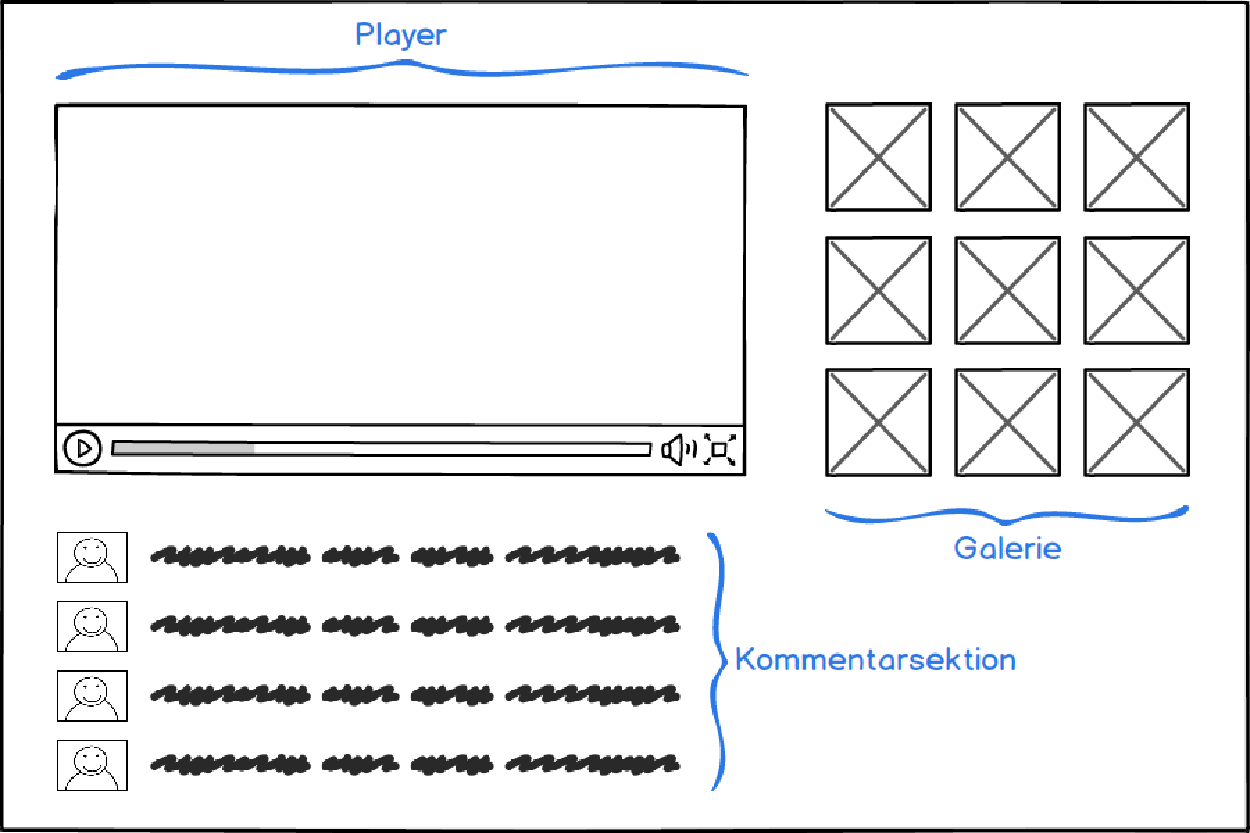
\includegraphics[width=.8\textwidth,center]{MockupBereiche.pdf}
\caption{\label{fig:MockupBereiche}Erste Skizze der Moodle-Repräsentation eines Hyperaudio-Dokuments}
\end{figure}

%Bevor nun die Bedürfnisse festgehalten werden, ist es zunächst sinnvoll das Plugin in mehrere Bereiche aufzuteilen. Hierbei scheint die Aufteilung in die Bereiche Schnittstelle, Integration in die Moodle-Oberfläche, Player für Hyperaudio-Dokumente und Kommentarfunktion plausibel.

%%%%%%%%%%
\section{Bedürfnisse der Studierenden und Lehrenden}
Bevor wir mit der detaillierten Konzeption des Plugins beginnen können, ist es wichtig, sich nochmals genauer mit den möglichen Bedürfnissen der Studierenden und Lehrenden auseinanderzusetzen. Eine Analyse der Bedürfnisse mittels Umfrage und/oder Interviews würde den Umfang dieser Arbeit sprengen, weshalb hierauf verzichtet wird.

Nun sollen im ersten Schritt die Anforderungen an die einzelnen Bereiche erarbeitet werden, wobei bereits die Gruppe der Betroffenen mit festgehalten werden soll. Nachdem die Anforderungen erfasst wurden, sollen diese im zweiten Schritt mit einer Priorität versehen werden. Diese wird dann herangezogen um bei der geplanten iterativen Programmierung die Reihenfolge, in der die Anforderungen umgesetzt werden, zu bestimmen.

%%%%%%%%%%
\subsection{Anforderungen an die Schnittstelle}
Die Schnittstelle soll es den Lehrenden ermöglichen, Hyperaudio-Dokumente in Moodle zu übertragen. Um die Anforderungen an die Schnittstelle zu ermitteln, überlegen wir kurz was ein Hyperaudio-Dokument ausmacht. Ein solches Dokument besteht zum einen aus einer Audio-Datei. Hieraus resultiert die Anforderung an die Schnittstelle, dass man festlegen können muss, welche Audio-Datei abgespielt werden soll. Zum anderen besteht ein Hyperaudio-Dokument aus zeitabhängigen Annotationen von Bildern, Tabellen, Formeln etc. Die Schnittstelle muss es uns also ermöglichen, zu definieren, zu welchem Zeitpunkt und für welche Dauer welches Zusatzinhalte angezeigt werden soll. Außerdem wäre es noch praktisch, Metadaten, wie den Autor, Quellen oder weiterführende Links, an das Hyperaudio-Dokument anzuheften. Um all diese Informationen zu speichern entsteht automatisch die Anforderung an eine Schnittstellen-Datei. Natürlich muss es auch die Möglichkeit geben, das Hyperaudio-Dokument in Moodle zu importieren. Alle diese Anforderungen (siehe Tabelle \ref{tab:AnforderungenSchnittstelle}) haben gemeinsam, dass ausschließlich die Lehrenden die Betroffenen darstellen.

\begin{table}[!ht]
\def\arraystretch{1.4}
\caption{Anforderungen an die Schnittstelle}
\label{tab:AnforderungenSchnittstelle}
 \begin{tabularx}{\textwidth}{lXl}      
    \hline
    Nr. & Anforderung & Betroffene 
    \\\hline
    1. & Definition einer Schnittstellen-Datei & \\
    1.1 & Definition der abzuspielenden Audiodatei & Lehrende\\
    1.2 & Definition der zeitabhängigen Annotationen (Bildern, Tabellen, Formeln etc.) & Lehrende\\
    1.3 & Definition von Metadaten (Autor, Quellen, weiterführende Links etc.) & Lehrende\\
    2. & Entwickeln eines Imports für Moodle & Lehrende\\
    \hline
    \end{tabularx}
\end{table}

%%%%%%%%%%
\subsection{Anforderungen an die Integration in die Moodle-Oberfläche}
\label{sub:AnforderungenOberflaeche}
Um die Anforderungen für die Integration in die Moodle-Oberfläche (siehe Tabelle \ref{tab:AnforderungenIntegration}) zu bestimmen, versuchen wir uns in die Studierenden und Lehrenden hineinzuversetzen. 

Zunächst beginnen wir mit der Perspektive der Lehrenden. Für diese Gruppe steht natürlich die Administration von Hyperaudio-Dokumenten im Vordergrund. Dementsprechend muss eine Administrationsseite zur Verfügung gestellt werden, über welche die Hyperaudio-Dokumente hochgeladen und verwaltet werden können.

Nun kommen wir zu den Anforderungen, die sowohl Lehrende als auch Studierende an die Integration stellen. Die zentrale Anlaufstelle, an denen die Lerninhalte für die Lehrenden und Studierenden angezeigt werden, ist natürlich die Kursseite des jeweiligen Kurses. Also muss die Darstellung der Hyperaudio-Dokumente in die Kursseiten integriert werden. Bei dieser Integration müssen wiederum neben der reinen Integration eines Players für Hyperaudio-Dokumente weitere Aspekte berücksichtigt werden. Eine weitere Anforderung könnte sein, dass alle dargestellten Zusatzinhalte in einer separaten Galerie dargestellt werden, damit sich schnell einen Überblick über diese gemacht werden kann und gegebenenfalls schnell wieder an die entsprechende Stelle im Hyperaudio-Dokument gesprungen werden kann. Hier ist also auch eine Rückkopplung zum Player notwendig. Des Weiteren muss hier auch die gewünschte Kommentarsektion eingebunden werden, über welche sich die Studierenden und Lehrenden untereinander austauschen können.

Zusätzlich ist auch eine Favoritenfunktion denkbar, mit welcher sich Studierende und Lehrende bestimmte Hyperaudio-Dokumente als Favoriten speichern können. Passend hierzu müsste es dann eine Übersicht über alle favorisierten Hyperaudio-Dokumente geben, welche ähnlich dargestellt werden könnte wie die bereits vorhandene Moodle-Ansicht \glqq Meine Lernumgebungen\grqq.

Eine Übersicht über alle zuletzt abgespielten Dokumente stellt eine ähnliche Anforderung dar.

Eine weitere mögliche Anforderung ist eine Übersichtsseite über alle verfügbaren Hyperaudio-Angebote aufgegliedert nach Kurs, Kurseinheit und Kapitel.

\begin{table}[!ht]
\def\arraystretch{1.4}
\caption{Anforderungen an die Integration in die Moodle-Oberfläche}
\label{tab:AnforderungenIntegration}
 \begin{tabularx}{\textwidth}{lXl}      
    \hline
    Nr. & Anforderung & Betroffene 
    \\\hline
    1. & Einbindung der Administration in die Kursseite & Lehrende\\
    2. & Einbindung der Hyperaudio-Dokumente in die Kursseite & \\
    2.1 & Einbindung des Players & Lehrende und Studierende\\
    2.2 & Einbindung einer Galerie der zeitabhängig annotierten Bilder, Tabellen, Formeln etc. mit Rückkopplung zum Player & Lehrende und Studierende\\
    2.3 & Einbindung der Kommentarsektion & Lehrende und Studierende\\
    3. & Favoritenfunktion analog zu \glqq Meine Lernumgebungen\grqq & Lehrende und Studierende\\
    4. & Übersicht über zuletzt abgespielte Hyperaudio-Dokumente & Lehrende und Studierende\\
    5. & Übersicht über alle verfügbaren Hyperaudio-Angebote & Lehrende und Studierende\\
    \hline
    \end{tabularx}
\end{table}

%%%%%%%%%%
\subsection{Anforderungen an die Kommentarsektion}
\label{sub:AnforderungenKommentarsektion}
Nachdem bereits bei den Anforderungen an die Intergration in die Moodle-Oberfläche auf die Kommentarsektion verwiesen wurde, sollen nun auch hierfür die Anforderungen definiert werden. Zunächst besteht der Wunsch, dass die Kommentarsektion neben öffentlichen Kommentaren auch persönliche Notizen enthalten können soll.

An dieser Stelle wollen wir die Unterscheidung zwischen öffentlichen Kommentaren, persönlichen Notizen und persönlichen Markierungen vornehmen. Öffentliche Kommentare stellen die übliche Art der Kommentare dar, mittels derer der Austausch unter den Studierenden und den Lehrenden stattfindet. Persönliche Notizen stellen eine spezielle Form der Kommentare dar. Diese sind im Grunde auf gleiche Art und Weise wie die öffentlichen Kommentare zu verstehen, mit der einzigen Ausnahme, dass diese nur durch den Verfasser eingesehen werden können. Persönliche Markierungen dagegen sollen dem Studierenden oder Lehrenden die Möglichkeit geben, bestimmte Zeitpunkte des Hyperaudio-Dokuments für eventuelle spätere Bearbeitungen vorzumerken. Markierungen werden nur innerhalb des Players vorgenommen, sodass diese keinen Bestandteil der Kommentarsektion darstellen. %Persönliche Markierungen dagegen sollen dem Studierenden und Lehrenden die Möglichkeit geben, eine im Player sichtbare Markierung innerhalb der Fortschrittsleiste vorzunehmen. Diese Markierungen stellen also keinen Bestandteil der Kommentarsektion dar.

%Am Anfang steht hier zunächst die Anforderung, dass Kommentare und persönliche Notizen erstellt werden können. Diese Kommentare und persönlichen Notizen sollen in der Kommentarsektion chronologisch dargestellt werden.
In der Kommentarsektion sollen Kommentare und Notizen chronologisch dargestellt werden.
% Dabei soll aus zwei Betrachtungsweisen entschieden werden können, zum einen der Betrachtung anhand des Erstellungsdatums und zum anderen mittels des Zeitpunktes zu dem der Kommentar oder die Notiz an das Hyperaudio-Dokument annotiert wurde.
Die Sortierung erfolgt standardmäßig anhand der Zeitpunkte, zu denen die Kommentare oder Notizen an das Hyperaudio-Dokument annotiert wurden. Alternativ kann der Betrachter auch eine Sortierung nach Erstellungsdatum wählen. 
Da die Studierenden und Lehrenden sich mittels der Kommentare austauschen können sollen, besteht auch die Anforderung, direkt auf einen öffentlichen Kommentar antworten zu können. Bei persönlichen Notizen besteht der Wunsch, diese auch bearbeiten und löschen zu können. Da jeder Kommentar und auch jede Notiz zu einem bestimmten Zeitpunkt innerhalb des Hyperaudio-Dokuments gehört, soll es auch möglich sein, vom jeweiligen Kommentar beziehungsweise von der jeweiligen Notiz aus zu der entsprechenden Stelle im Hyperaudio-Dokument zu springen. Diese Anforderung wird entsprechend in Tabelle \ref{tab:AnforderungenKommentarsektion} ergänzt. Zusätzlich wäre es auch von Vorteil, wenn in den Kommentare und Notizen nach Stichwörtern gesucht werden könnte.

\begin{table}[!ht]
\def\arraystretch{1.4}
\caption{Anforderungen an die Kommentarsektion}
\label{tab:AnforderungenKommentarsektion}
 \begin{tabularx}{\textwidth}{lXl}      
    \hline
    Nr. & Anforderung & Betroffene 
    \\\hline
    %1. & Erstellen von Kommentaren und persönlichen Notizen & Lehrende und Studierende\\
    1. & Chronologische Darstellung der Kommentare und Notizen & Lehrende und Studierende\\
    2. & Antworten auf öffentliche Kommentare & Lehrende und Studierende\\
    3. & Bearbeiten persönlicher Notizen & Lehrende und Studierende\\
    4. & Löschen persönlicher Notizen & Lehrende und Studierende\\
    5. & Rückkopplung zum Player & Lehrende und Studierende\\
    6. & Suchfunktion in den Kommentaren und Notizen & Lehrende und Studierende\\
    \hline
    \end{tabularx}
\end{table}

%%%%%%%%%%
\subsection{Anforderungen an den Player für Hyperaudio-Dokumente}
Wenden wir uns nun den Anforderungen an den Player zu. Hierbei macht es wieder Sinn sich zu überlegen was mit dem Hyperaudio-Dokument bezweckt werden soll. Die Grundfunktion des Players besteht darin, Audio-Dateien abzuspielen. Zusätzlich sollen die zeitabhängig annotierten Zusatzinhalte dargestellt werden. Zu dem Zeitpunkt, zu dem die Zusatzinhalte dargestellt werden, ist die Wiedergabe eines \textit{Audio Cues}, also eines akustischen Hinweises, gewünscht, der die Zuhörer auf die Anzeige der annotierten Zusatzinhalte aufmerksam macht. Eine weitere Anforderung ist die Einbettung der Kommentare und Notizen in den Player. Diese besteht zum einen aus der reinen Visualisierung der zeitabhängig annotierten Kommentare und Notizen, zum anderen werden auch Interaktionsmöglichkeiten geboten, sei es die Weiterleitung an die entsprechende Stelle in der Kommentarsektion oder die Erstellung neuer zeitabhängiger annotierter Kommentare und Notizen.  Auch das Erstellen und Löschen von persönlichen Markierungen innerhalb des Players samt derer Visualisierung stellt eine Anforderung an den Player dar und wird in Tabelle \ref{tab:AnforderungenPlayer} festgehalten.

Vorstellbar ist darüber hinaus, dass der Player sich beim Schließen der Seite merkt, zu welchem Zeitpunkt das Hyperaudio-Dokument beendet wurde, um es beim erneuten Öffnen an ebendieser Stelle fortzusetzen.

\begin{table}[!ht]
\def\arraystretch{1.4}
\caption{Anforderungen an den Player für Hyperaudio-Dokumente}
\label{tab:AnforderungenPlayer}
 \begin{tabularx}{\textwidth}{lXl}      
    \hline
    Nr. & Anforderung & Betroffene 
    \\\hline
    1. & Wiedergabe der Audiodatei & Lehrende und Studierende\\
    2. & Darstellung der zeitabhängig annotierten Bilder, Tabellen, Formeln etc & Lehrende und Studierende\\
    3. & Wiedergabe der Audio Cues & Lehrende und Studierende\\
    4. & Einbettung der Kommentare und Notizen & \\
    4.1 & Visualisierung der zeitabhängig annotierten Kommentare und Notizen & Lehrende und Studierende\\
    4.2. & Interaktionsmöglichkeiten & \\
    4.2.1 & Weiterleitung zu vorhandenen Kommentaren und Notizen in der Kommentarsektion  & Lehrende und Studierende\\
    4.2.2 & Erstellen zeitabhängiger annotierter Kommentare und Notizen & Lehrende und Studierende\\
    5. & Einbettung der persönlichen Markierungen & \\
    5.1 & Visualisierung der zeitabhängig annotierten Markierungen & Lehrende und Studierende\\
    5.2. & Interaktionsmöglichkeiten & \\
    5.2.1 & Erstellen zeitabhängig annotierter Markierungen  & Lehrende und Studierende\\
    5.2.2 & Löschen zeitabhängig annotierter Markierungen & Lehrende und Studierende\\
    6. & Funktion zum Fortsetzen unterbrochener Wiedergaben bei folgenden Aufrufen in Moodle & Lehrende und Studierende\\
    \hline
    \end{tabularx}
\end{table}

%%%%%%%%%%
\subsection{Priorisierung der Anforderungen}
Im nächsten Schritt nehmen wir die Priorisierung der erfassten Anforderungen vor. Hierbei wird bewertet wie wichtig der in der Anforderung beschriebene Wunsch für die Erreichung des Lernziels ist. Die Priorisierung wird anhand der drei Prioritätsstufen \textit{niedrig}, \textit{mittel} und \textit{hoch} festgelegt.

\subsubsection{Priorisierung: Anforderungen an die Schnittstelle}
Wenn die gesammelten Anforderungen an die Schnittstelle betrachtet werden, kann festgestellt werden, dass abgesehen von der Definition von Metadaten (Autor, Quellen, weiterführende Links etc.) alle Anforderungen essenziell für die Erreichung des Lernziels und somit zur Umsetzung des Plugins sind. Die Metadaten stellen aber dennoch sinnvolle Informationen bereit, welche dem Studierenden beim Erreichen des Lernziels helfen können. Daraus resultiert die in Tabelle \ref{tab:PriorisierungAnforderungenSchnittstelle} dargestellte Priorisierung.

\begin{table}[!ht]
\def\arraystretch{1.4}
\caption{Priorisierung: Anforderungen an die Schnittstelle}
\label{tab:PriorisierungAnforderungenSchnittstelle}
 \begin{tabularx}{\textwidth}{lXll}      
    \hline
    Nr. & Anforderung & Betroffene & Priorität
    \\\hline
    1. & Definition einer Schnittstellen-Datei & & \\
    1.1 & Definition der abzuspielenden Audiodatei & Lehrende & hoch\\
    1.2 & Definition der zeitabhängigen Annotationen (Bildern, Tabellen, Formeln etc.) & Lehrende & hoch\\
    1.3 & Definition von Metadaten (Autor, Quellen, weiterführende Links etc.) & Lehrende & mittel\\
    2. & Entwickeln eines Imports für Moodle & Lehrende & hoch\\
    \hline
    \end{tabularx}
\end{table}

%%%%%%%%%%
\subsubsection{Priorisierung: Anforderungen an die Integration in die Moodle-Oberfläche}
Bei der Integration in die Moodle-Oberfläche ergibt sich eine Priorisierung in drei Stufen. Auf die Einbindung der Administration in die Kursseite kann nicht verzichtet werden, genauso wie auf die Einbindung der Hyperaudio-Dokumente in die Kursseite inklusive des Players und der Kommentarsektion. Demzufolge erhalten diese Anforderungen die Priorität \textit{hoch}. Der Anforderung \glqq Einbindung einer Galerie der zeitabhängig annotierten Bilder, Tabellen, Formeln etc. mit Rückkopplung zum Player\grqq{} wird die Priorität \textit{mittel} zugeordnet, da sie das Erreichen des Lernziels sehr wohl unterstützen kann, aber nicht zwangsweise dafür benötigt wird. Alle weiteren Anforderungen an die Integration in die Moodle-Oberfläche werden mit der Priorität \textit{niedirg} in Tabelle \ref{tab:PriorisierungAnforderungenIntegration} festgehalten, da sie nicht dem eigentlichen Erreichen des Lernziels dienen, sondern nur eine verbesserte Übersicht über die Hyperaudio-Dokumente bieten.

\begin{table}[!ht]
\def\arraystretch{1.4}
\caption{Priorisierung: Anforderungen an die Integration in die Moodle-Oberfläche}
\label{tab:PriorisierungAnforderungenIntegration}
 \begin{tabularx}{\textwidth}{lXll}      
    \hline
    Nr. & Anforderung & Betroffene & Priorität
    \\\hline
    1. & Einbindung der Administration in die Kursseite & Lehrende & hoch\\
    2. & Einbindung der Hyperaudio-Dokumente in die Kursseite & \\
    2.1 & Einbindung des Players & Lehrende und Studierende & hoch\\
    2.2 & Einbindung einer Galerie der zeitabhängig annotierten Bilder, Tabellen, Formeln etc. mit Rückkopplung zum Player & Lehrende und Studierende & mittel\\
    2.3 & Einbindung der Kommentarsektion & Lehrende und Studierende & hoch\\
    3. & Favoritenfunktion analog zu \glqq Meine Lernumgebungen\grqq & Lehrende und Studierende & niedrig\\
    4. & Übersicht über zuletzt abgespielte Hyperaudio-Dokumente & Lehrende und Studierende & niedrig\\
    5. & Übersicht über alle verfügbaren Hyperaudio-Angebote & Lehrende und Studierende & niedrig\\
    \hline
    \end{tabularx}
\end{table}

%%%%%%%%%%
\subsubsection{Priorisierung: Anforderungen an die Kommentarsektion}
Der Hauptbestandteil der Kommentarsektion besteht aus der Darstellung der Kommentare und Notizen. Die Vergabe einer hohen Priorität für diese Anforderung (siehe Tabelle \ref{tab:PriorisierungAnforderungenKommentarsektion}) ist daher trivial. Die Möglichkeit direkt auf Kommentare zu antworten und die Möglichkeit persönliche Notizen zu löschen stellen sinnvolle Erweiterungen der Kommentarfunktion dar, welche das Erreichen des Lernziels erleichtern können. Dies rechtfertigt die Priorität \textit{mittel}. Dem Bearbeiten persönlicher Notizen wird die Priorität \textit{niedrig} zugewiesen, da dieselben Ergebnisse auch dadurch erzielt werden können, dass ein bestehender Kommentar gelöscht und ein neuer Kommentar erstellt wird. Eine Bearbeitungsfunktion eröffnet also keine neuen Möglichkeiten, stellt jedoch eine Erleichterung des Arbeitsschrittes dar. Der Anforderung \glqq Rückkopplung zum Player\grqq{} wird die Priorität \textit{mittel} zugeordnet, da sie, ähnlich wie die Galerie, das Erreichen des Lernziels unterstützen kann, aber nicht zwangsweise dafür benötigt wird.
%Da der Fokus bei den Kommentaren von Hyperaudio-Dokumenten auf der Zeit und nicht direkt auf dem Inhalt liegt wird der Suchfunktion nur eine geringe Priorität zugewiesen
Eine Suchfunktion innerhalb der Kommentare ist nützlich, um Inhalte zu bestimmten Themen zu finden. Die Kommentare können jedoch auch anhand der Visualisierung im Player oder über die Inhalte der Galerie angesteuert werden. Da die Suchfunktion demnach nicht die einzige Möglichkeit darstellt, um zu den gewünschten Kommentaren zu navigieren, wird dieser nur eine geringe Priorität zugewiesen.

\begin{table}[!ht]
\def\arraystretch{1.4}
\caption{Priorisierung: Anforderungen an die Kommentarsektion}
\label{tab:PriorisierungAnforderungenKommentarsektion}
 \begin{tabularx}{\textwidth}{lXll}      
    \hline
    Nr. & Anforderung & Betroffene & Priorität
    \\\hline
    %1. & Erstellen von Kommentaren und persönlichen Notizen & Lehrende und Studierende & hoch\\
    1. & Chronologische Darstellung der Kommentare und Notizen & Lehrende und Studierende & hoch\\
    2. & Antworten auf öffentliche Kommentare & Lehrende und Studierende & mittel\\
    3. & Bearbeiten persönlicher Notizen & Lehrende und Studierende & niedrig\\
    4. & Löschen persönlicher Notizen & Lehrende und Studierende & mittel\\
    5. & Rückkopplung zum Player & Lehrende und Studierende & hoch\\
    6. & Suchfunktion in den Kommentaren und Notizen & Lehrende und Studierende & niedrig\\
    \end{tabularx}
\end{table}

%%%%%%%%%%
\subsubsection{Priorisierung: Anforderungen an den Player für Hyperaudio-Dokumente}
Beim Player stellen die Wiedergabe der Audiodatei und die Darstellung der zeitabhängig annotierten Bilder, Tabellen, Formeln etc. die essenziellen Funktionen dar und werden entsprechend mit der Priorität \textit{hoch} bewertet. Mit dem Hintergrund, dass die Studierenden während des Abspielens des Hyperaudio-Dokuments andere Tätigkeiten ausüben können und nur in bestimmen Momenten auf den PC blicken müssen sollen, kann auch die Anforderung \glqq Wiedergabe der Audio Cues\grqq{} mit der Priorität \textit{hoch} bedacht werden. Es ist zu betonen, dass die Kommentarfunktion einen wesentlichen Bestandteil des Plugins ausmachen soll. Um die Nutzung der Kommentarfunktion beim Abspielen der Dokumente möglichst komfortabel zu gestalten, sollten die Interaktionsmöglichkeiten entsprechend mit der Priorität \textit{hoch} versehen werden. Gleiches gilt für die Anforderungen bezüglich der persönlichen Markierungen. Die Visualisierung der Kommentare, Notizen und Markierungen an sich wird ebenfalls mit der Priorität \textit{hoch} bewertet.
% Das Erreichen des Lernzieles wird dadurch erleichtert, dass beim Abspielen des Dokuments schnell die gewünschten Aktionen ausgeführt werden können und somit weniger kostbare Lernzeit verschwendet wird.
Durch die Umsetzung der eben genannten Anforderungen können beim Abspielen des Dokuments schnell die gewünschten Aktionen ausgeführt werden, wodurch letztlich das Erreichen des Lernzieles erleichert wird.
Der Funktion zum Fortsetzen unterbrochener Wiedergaben bei folgenden Aufrufen in Moodle wird eine geringere Bedeutung zugeschrieben, da falls gewünscht beispielsweise auch mittels einer persönlichen Notiz oder Markierung der Zeitpunkt festgehalten werden kann, an dem das Dokument beim nächsten Aufruf fortgesetzt werden soll. Dementsprechend wird dieser Anforderung in Tabelle \ref{tab:PriorisierungAnforderungenPlayer} nur eine geringe Priorität zugeordnet.

\begin{table}[!ht]
\def\arraystretch{1.4}
\caption{Priorisierung: Anforderungen an den Player für Hyperaudio-Dokumente}
\label{tab:PriorisierungAnforderungenPlayer}
 \begin{tabularx}{\textwidth}{lXll}      
    \hline
    Nr. & Anforderung & Betroffene & Priorität
    \\\hline
    1. & Wiedergabe der Audiodatei & Lehrende und Studierende & hoch\\
    2. & Darstellung der zeitabhängig annotierten Bilder, Tabellen, Formeln etc. & Lehrende und Studierende & hoch\\
    3. & Wiedergabe der Audio Cues & Lehrende und Studierende & hoch\\
    4. & Einbettung der Kommentare und Notizen & \\
    4.1 & Visualisierung der zeitabhängig annotierten Kommentare und Notizen & Lehrende und Studierende & hoch\\
    4.2. & Interaktionsmöglichkeiten & \\
    4.2.1 & Weiterleitung zu vorhandenen Kommentaren und Notizen in der Kommentarsektion  & Lehrende und Studierende & hoch\\
    4.2.2 & Erstellen zeitabhängiger annotierter Kommentare und Notizen & Lehrende und Studierende & hoch\\
    5. & Einbettung der persönlichen Markierungen & \\
    5.1 & Visualisierung der zeitabhängig annotierten Markierungen & Lehrende und Studierende & hoch\\\\
    5.2. & Interaktionsmöglichkeiten & \\
    5.2.1 & Erstellen zeitabhängig annotierter Markierungen  & Lehrende und Studierende & hoch\\
    5.2.2 & Löschen zeitabhängig annotierter Markierungen & Lehrende und Studierende & hoch\\
    6. & Funktion zum Fortsetzen unterbrochener Wiedergaben bei folgenden Aufrufen in Moodle & Lehrende und Studierende & niedrig\\
    \hline
    \end{tabularx}
\end{table}

%%%%%%%%%%
\section{Lernen mit Hypermedia}
Bevor wir uns der genauen Konzeption und Implementation des Moodle Plugins für Hyperaudio-Dokumente zuwenden, betrachten wir zunächst \textit{Hypermedia} im Allgemeinen. Dabei wollen wir zunächst eine Begriffsklärung durchführen. Darauf aufbauend werden einige Erfahrungen aus verschiedenen wissenschaftlichen Arbeiten gesammelt. Zuletzt wollen wir hieraus einige Rückschlüsse für unser Moodle Plugin und unsere Interpretation von Hyperaudio ziehen.

%%%%%%%%%%
\subsection{Begriffsklärung}
Hyperaudio stellt eine Ausprägung von \textit{Hypermedia} dar. Der Begriff \textit{Hypermedia} wurde das erste Mal von Ted Nelson 1965 verwendet \citep{nelson1965complex}. In seinem Paper beschreibt er detailliert, was er sich unter einem \textit{Hypertext} vorstellt. Hierunter versteht er ein Dokument bestehend aus geschriebenen oder bildhaften Inhalten, welche in solch einer komplexen Art und Weise miteinander verbunden sind, dass sie nicht mehr auf Papier dargestellt werden können. Es kann Zusammenfassungen, Karten über die Inhalte und deren Zusammenhänge, Annotationen, Ergänzungen oder Anmerkungen von Wissenschaftlern, die das Dokument begutachtet haben, enthalten. Nelson beschreibt das Kriterium für den Präfix \textit{hyper} damit, dass diese Objekte nicht durch eine Konvertierung in ein einfaches lineares Medium, wie beispielsweise einen String umgewandelt werden können. Der wesentliche Punkt ist also, dass es sich beim Lernen mit \textit{Hypermedia} um ein nicht-lineares Lernen handelt.

Genauer betrachtet stellt das, was Nelson sich damals als \textit{Hypertext} vorgestellt hatte, nach heutiger Definition bereits eine Form von \textit{Hypermedia} dar. Auch wenn viele die beiden Begriffe \textit{Hypertext} und \textit{Hypermedia} synonym verwenden \citep{nielsen2013multimedia}, werden bei strikter Betrachtung bei \textit{Hypertext} ausschließlich Texte miteinander verbunden, während bei \textit{Hypermedia} auch andere Medien eingebunden werden können. Gemeinsam haben beide Arten jedoch, dass der Lernende keinen linearen Weg vorgegeben hat, sondern von einem Knoten (Node) zum anderen springen kann und sich somit seinen Lernweg selbst aussucht. Als Folge dessen stellt \textit{Hypermedia} eine nicht-lineare Variante von \textit{Multimedia} dar.

Nach dieser Logik handelt es sich bei Hyperaudio in seiner klassischen Form eigentlich um reine Audiosequenzen, die miteinander verknüpft sind, wobei der Lernende selbst entschieden kann, in welcher Reihenfolge er diese abspielt \citep{zumbach2006learning}.

%%%%%%%%%%
\subsection{Erfahrungen}
Die Wissenschaft beschäftigt sich schon seit vielen Jahren damit, festzustellen, welche Effekte der Einsatz von \textit{Multimedia}, \textit{Hypertext} und \textit{Hypermedia} auf den Lernerfolg von Lehrenden hat. In der Arbeit von \cite{moos2010multimedia} wird eine Analyse von etlichen Arbeiten zu diesem Thema durchgeführt. \cite{moos2010multimedia} konzentrieren sich hierbei vor allem auf den Einfluss auf die Motivation der Lernenden. Dennoch wird auch auf andere Aspekte der drei verschiedenen E-Learning Methoden \textit{Multimedia}, \textit{Hypertext} und  \textit{Hypermedia} im Vergleich zu klassischen Lehrmethoden eingegangen.

\cite{moos2010multimedia} verweisen auf Arbeiten, nach denen eine Herausforderung bei \textit{Multimedia} und somit auch bei \textit{Hypermedia} darin besteht, dass die kognitive Aufnahmekapazität der Studierenden überschritten werden kann (Mayer und Moreno; van Merrienboer und Ayres, nach \cite{moos2010multimedia}), wenn Informationen sowohl aus einem Text als auch aus einem Diagramm entnommen werden sollen. Dies beruht auf der Annahme der Cognitive Load Theory, welche dem Arbeitsgedächtnis nur eine begrenzte Kapazität zuspricht (Sweller; van Merrienboer und Sweller, nach \cite{moos2010multimedia}). Es gibt aber auch Studien, welche einen positiven Effekt nachweisen, wenn zur gleichen Zeit Bilder dargestellt werden und dazu passender Text vorgelesen wird, im Vergeleich zum alleinigen Betracheten von Bildern beziehungsweise Anhören von Texten (Mayer und Anderson; Mayer und Sims, nach \cite{moos2010multimedia}).

\textit{Hypertext} bietet zwar Vorteile, da der Studierende den Lernweg bestimmen kann, der am besten auf seine Bedürfnisse angepasst ist. Auf der anderen Seite ist hierzu aber eine ausreichende Vorkenntnis in dem Lernbereich notwendig, um die Entscheidung, wie dieser Weg aussehen soll treffen zu können. Des Weiteren wirkt sich auch ein fehlendes Interesse des Studierenden negativ auf die Effektivität der \textit{Hypertext} Lernumgebung aus (Lawless und Kulikowich, nach \cite{moos2010multimedia}).
\todo[inline]{Zitat nochmals prüfen}

Es ist nun also nicht verwunderlich, dass \textit{Hypermedia} als Verschmelzung von \textit{Multimedia} und \textit{Hypertext} ebenfalls einige Herausforderungen mit sich bringt \citep{moos2010multimedia}. Scott und Schwartz (nach \cite{moos2010multimedia}) fordern für das Lernen mit \textit{Hypermedia} eine Balance zwischen effektiver Navigation und Inhaltsverständnis. Dies soll durch Prozesse zur Überwachung des eigenen Lernfortschritts erreicht werden, doch Untersuchungen haben ergeben, dass viele Studierende Schwierigkeiten haben diese Prozesse korrekt anzuwenden \citep{moos2010multimedia}.


%%%%%%%%%%
\subsection{Rückschlüsse}
Nachdem wir nun die Begrifflichkeiten um \textit{Hypermedia}, sowie den Begriff Hyperaudio im eigentlichen Sinne beleuchtet und entsprechende Studien betrachtet haben, gehen wir nun darauf ein, welche Rückschlüsse daraus für diese Arbeit gezogen werden können.

Zum einen stellen wir fest, dass wir den Begriff Hyperaudio nicht im ursprünglichen Sinn verwenden. Bei unseren Hyperaudio-Dokumenten handelt es sich eigentlich um Multimedia-Dokumente. Erst unter Berücksichtigung der Kommentarfunktion und der Galerie wird der Hypermedia-Aspekt erfüllt. Der Zuhörer hat also die Möglichkeit von Kommentar zu Kommentar oder von Annotation zu Annotation zu springen und gelangt dabei an die entsprechende Stelle in der Audiosequenz. Im Gegensatz zu \cite{zumbach2006learning} verstehen wir unter Hyperaudio eine Audio-Datei, die durch die Erweiterung mittels Annotationen und Kommentarfunktion um Multimedia- und Hypermedia-Elemente ergänzt wird.

Der Vorteil unserer Betrachtungsweise von Hyperaudio liegt darin, dass die Herausforderungen, die in Verbindung mit \textit{Hypermedia} bzw. \textit{Hypertext} normalerweise auftreten, nicht besonders prägnant sind. In unserem Plugin wird dem Studierenden in erster Linie eine lineare Audio-Datei vorgespielt, die um Multimedia-Elemente ergänzt wird. Erst durch den Einsatz der Galerie und der Kommentarfunktion kommen die herausfordernden Elemente von Hypermedia ins Spiel. Dementsprechend sollte unser Hyperaudio-Plugin einen guten Kompromiss zwischen den verschiedenen Lehrmethoden darstellen.

%%%%%%%%%%
\section{Zusammenhänge der medialen Komponenten von Hyperaudio-Dokument und Annotationen}
In diesem Abschnitt wollen wir nochmals genauer auf den Aufbau eines Hyperaudio-Dokuments im Sinne dieser Arbeit eingehen. Hierbei soll vor allem geklärt werden, wie die einzelnen Komponenten zusammenhängen und welche Möglichkeiten dadurch gegeben beziehungsweise nicht gegeben sind.

%%%%%%%%%%
\subsection{Komponenten}
Im Mittelpunkt eines Hyperaudio-Dokument steht eine Audio-Datei. Inhaltlich kann es sich hierbei beispielsweise um einen Vorlesungsvortrag handeln. Man könnte sich auch vorstellen, dass ein Hyperaudio-Dokument aus mehreren aneinandergereihten Audio-Dateien besteht. Dies würde an der grundsätzlichen Problemstellung jedoch nichts ändern und kann im Nachhinein jederzeit als Erweiterung umgesetzt werden. Aus diesem Grund wird in dieser Arbeit nur ein Plugin für ein Hyperaudio-Dokument bestehend aus einer Audio-Datei entwickelt.

Neben dieser zentralen Audio-Datei besteht das Hyperaudio-Dokument aus mehreren Zusatzinhalten, wobei es sich um Bilder, Graphen, Tabellen usw. handeln kann. Entscheidend ist aber, dass diese Zusatzinhalte immer nur eine rein grafische Darstellung verkörpern. Videos mit Ton sind somit beispielsweise nicht als Zusatzinhalt verwendbar, reine Animationen ohne Ton sind aber durchaus möglich.

Als besondere, nämlich externe Komponente, sind die Kommentare zu nennen. Diese gehören nicht zum eigentlichen Hyperaudio-Dokument, sollen aber mit diesem verknüpft werden. Es wird drei verschiedene Arten von Kommentaren geben, nämlich  öffentliche Kommentare, persönliche Notizen und persönliche Markierungen.  Innerhalb der öffentlichen Kommentare muss noch zwischen den Original-Kommentaren und den Antworten auf diese unterschieden werden. 


%%%%%%%%%%
\subsection{Zusammenhänge}
Zunächst betrachten wir den Zusammenhang zwischen Audio-Datei und den Zusatzinhalten. Zu jedem beliebigen Zeitpunkt innerhalb der Abspieldauer der Audio-Datei kann maximal ein Zusatzinhalt gleichzeitig annotiert werden. Es sind also auch Phasen möglich zu denen keinerlei Zusatzinhalt dargestellt wird. Das Zeitfenster für die Annotation soll mittels einer Start- und Endzeit pro Zusatzinhalt definiert werden, wobei nur die Minuten und Sekunden anzugeben sind. Bei dem Zeitfenster sollte natürlich bedacht werden, dass dieses nicht zu kurz sein sollte. Zwar soll, sobald ein Zusatzinhalt im Player des Hyperaudio-Dokuments angezeigt wird,  ein entsprechender Audio Cue abgespielt werden, dennoch können bereits einige Sekunden vergehen bis der Studierende seinen Blick dem Player zuwendet.

Auch die Kommentare stehen als externe Komponente in einer gewissen Art und Weise im Zusammenhang mit der Audio-Datei. Dies ergibt sich daraus, dass Kommentare zu einem bestimmten Zeitpunkt innerhalb der Audio-Datei erfasst werden. Während Antworten auf Original-Kommentare erfasst werden können, sind Antworten auf Antworten nicht möglich.

Zwischen Kommentaren und Zusatzinhalten gibt es jedoch keinen direkten Zusammenhang. Solche Zusammenhänge ergeben sich alleine aus den Zeitpunkten der Annotationen. Zusatzinhalte können wiederum in keinem Zusammenhang mit einem anderen Zusatzinhalt stehen.

Diese Zusammenhänge sind im UML-Diagramm in Abbildung \ref{fig:UMLAufbau} ersichtlich.

\begin{figure}[h!]
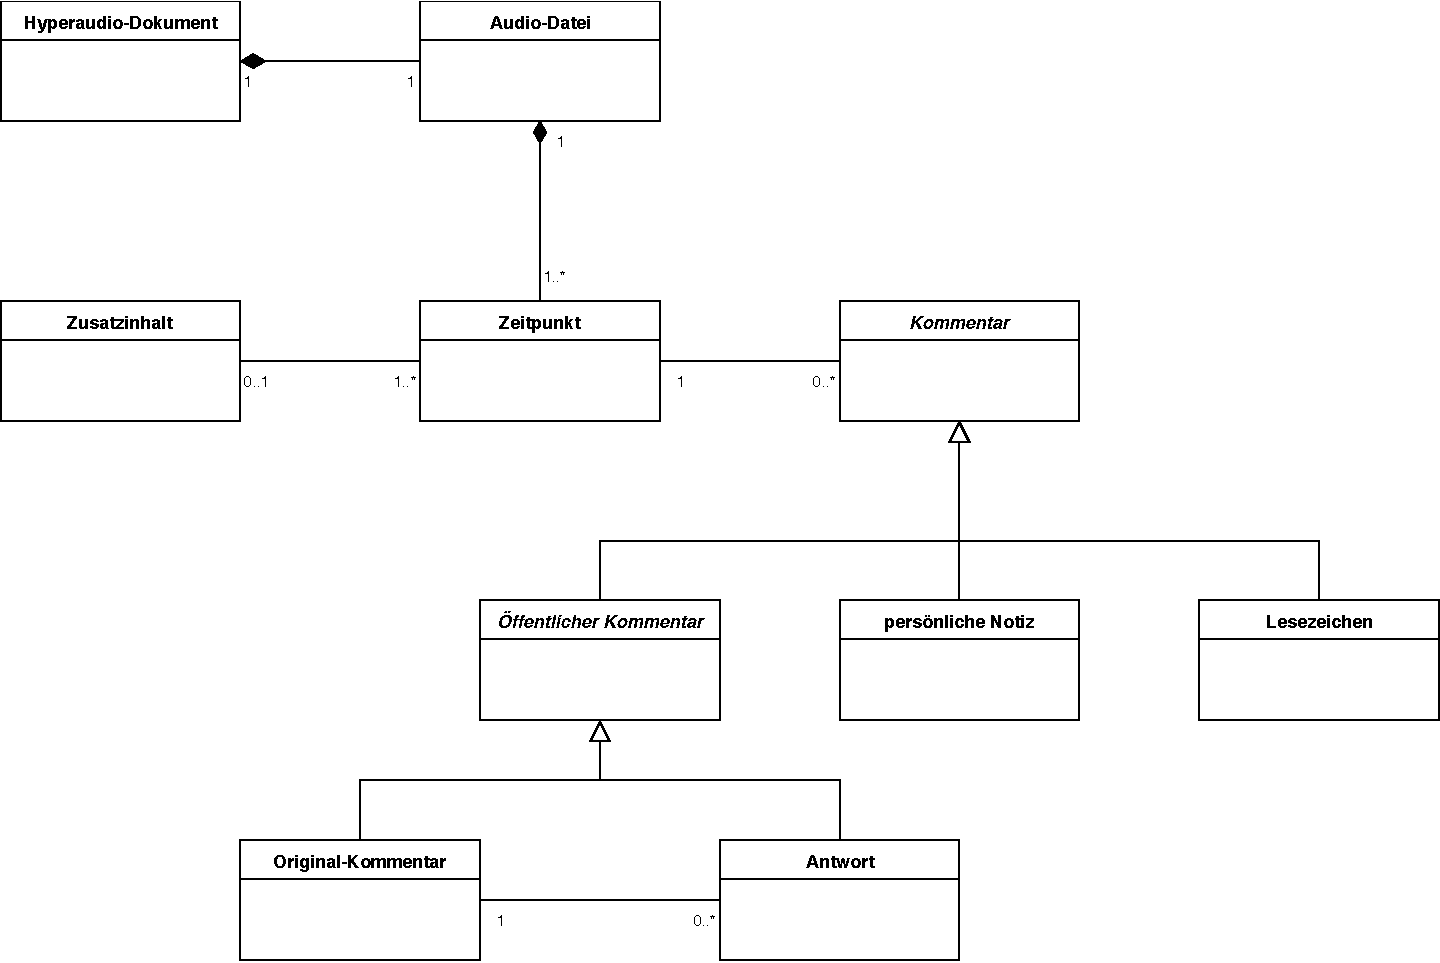
\includegraphics[width=\textwidth,center]{UMLZusammenhaenge.pdf}
\caption{\label{fig:UMLAufbau}Zusammenhänge der Komponenten}
\end{figure}


%%%%%%%%%%
\section{Evaluation bestehender Komponenten}
Bevor wir mit der Konzeption und Implementierung unseres Moodle-Plugins beginnen, wenden wir uns nun der Evaluation bestehender Komponenten zu. Ziel ist es festzustellen, ob eventuell bereits Technologien existieren, mit deren Hilfe unsere Idee des Moodle-Plugins umgesetzt werden kann oder ob zumindest Teile davon - unter entsprechender Beachtung der Lizenzierung - sinnvoll wiederverwendet werden können. Wir gehen hierbei so vor, dass wir die einzelnen vorhanden Technologien auf diesem Gebiet und ihre Funktionen vorstellen und anschließend bewerten, inwiefern diese für die Umsetzung des Plugins relevant sind.

%%%%%%%%%%
\subsection{VideoJS Player}
Bei dem \textit{VideoJS Player}\footnote{GitHub-Projekt, Apache-Lizenz 2.0: http://videojs.com/; https://github.com/videojs} handelt es sich um eine Open Source Bibliothek zum Abspielen von Videos und stellt damit einen HTML5 Video Player zur Verfügung. Der \textit{VideoJS Player} ist bereits als Standard Plugin für die Wiedergabe von Audio- und Video-Dateien in Moodle integriert. Wie der Name schon erkennen lässt, handelt es sich hierbei um eine JavaSrcipt Bibliothek. Der \textit{VideoJS Player} beschränkt sich in seiner Ausgangsversion ausschließlich auf das Abspielen von Audio- und Video-Dateien und bietet bis auf ein optionales Fallback auf den Adobe FlashPlayer keine weiteren Funktionen. Die Funktionalität des \textit{VideoJS Player} kann aber über Plugins erweitert werden. Es existieren bereits zahlreiche solcher Plugins. Hier sei vor allem das Plugin \textit{videojs-wavesurfer}\footnote{GitHub-Projekt, MIT Lizenz: https://github.com/collab-project/videojs-wavesurfer} zu nennen, welches das wavesurfer.js Framework (siehe Abschnitt \ref{sec:wavesurfer.js}) in den \textit{VideoJS Player} einbindet. Dank der Unterstützung von Plugins ist es durchaus denkbar, den Player mittels Plugin beispielsweise um Buttons zum Erstellen von Kommentaren oder persönlichen Notizen zu erweitern. Auch wäre es denkbar, mittels eines Plugins die annotierten Kommentare zu visualisieren. Grundsätzlich stellt der \textit{VideoJS Player} somit eine gute Ausgangslage für einen Hyperaudio-Player dar.

%%%%%%%%%%
\subsection{H5P}
Mit \textit{H5P} und dem bereits vorhanden Plugin für Moodle\footnote{GitHub-Projekt, GNU General Public License v2.0: https://github.com/h5p/h5p-moodle-plugin} ist es möglich, etliche verschieden Arten von interaktiven Lerninhalten zu gestalten. Dabei handelt es sich um eine Sammlung von interaktiven Komponenten, darunter Course Presentation, Timeline und Interactive Video. Course Presentation bietet die Möglichkeit, interaktive Präsentationen zu gestalten. Timeline kann genutzt werden um Inhalte anhand eines Zeitstrahls darzustellen. Interactive Video ermöglicht, ähnlich wie Course Presentation, die Interaktion während des Abspielens eines Videos. Besonders erwähnenswert ist, dass sich bei \textit{H5P} die interaktiven Inhalte innerhalb der Weboberfläche erstellen lassen. Es wäre also denkbar, eine eigene interaktive Komponente zu entwickeln, welche es ermöglicht, Hyperaudio-Dokumente als interaktiven Lerninhalt zu erstellen und abzuspielen.

%%%%%%%%%%
\subsection{Popcorn.js}
Die Mozilla Corporation bietet mit \textit{Popcorn.js}\footnote{GitHub-Projekt, MIT Lizenz: https://github.com/mozilla/popcorn-js} eine Bibliothek an, welche neben einer standardisierten Steuerung von Medieninhalten aus verschiedenen Quellen auch die Annotation von Inhalten mittels Plugins ermöglicht. Hier wäre also auch eine Entwicklung eines Plugins denkbar, mit welchem wir unsere Hyperaudio-Dokumente wie gewünscht wiedergeben könnten. Die Wartung für die Bibliothek wurde seitens Mozilla zwar eingestellt, das Projekt steht aber weiterhin auf GitHub zur Verfügung. Obwohl das Projekt nicht mehr weiterentwickelt wird, kann es durch die vorhandenen Steuerungsmöglichkeiten und das Plugin-System ein sehr geeignetes Grundgerüst für die Entwicklung unseres Moodle Plugins darstellen.
 
%%%%%%%%%%
\subsection{wavesurfer.js}
\label{sec:wavesurfer.js}
Bei \textit{wavesurfer.js}\footnote{GitHub-Projekt, BSD-3-Clause: https://wavesurfer-js.org; https://github.com/katspaugh/wavesurfer.js} handelt es sich um ein JavaScript Framework, welches es ermöglicht, die Wellenform zu der abgespielten Audio-Datei in einem Audio-Player visualisieren zu lassen. Diese Basisfunktionalität wurde durch Weiterentwicklungen um nützliche Funktionen erweitert. Auf zwei dieser Weiterentwicklungen gehen wir im Folgenden ein.

%%%%%%%%%%
\subsubsection{audio-annotator}
Der \textit{audio-annotator} stellt eine auf dem \textit{wavesurfer.js} Framework basierende Weiterentwicklung dar, welche es mittels Weboberfläche ermöglicht, Annotationen in Form von Text an eine Audio-Datei anzuheften. Es erweitert \textit{wavesurfer.js} also um die Möglichkeit, Annotationen an eine Datei anzuheften und bietet gleichzeitig noch eine Oberfläche, um ebendiese Annotationen vorzunehmen.

%%%%%%%%%%
\subsubsection{BAT - BMAT Annotation Tool}
Beim \textit{BAT - BMAT Annotation Tool}\footnote{GitHub-Projekt, GNU General Public License 3: https://wavesurfer-js.org; https://github.com/BlaiMelendezCatalan/BAT} handelt es sich um eine Entwicklung basierend auf der im Zusammenhang von \textit{audio-annotator} erweiterten Frameworks \textit{wavesurfer.js} und \textit{regions.js}. Es ermöglicht, ebenso wie \textit{audio-annotator}, dem Benutzer mittels Weboberfläche Annotationen an einer Audio-Datei vorzunehmen. Somit bietet \textit{BAT - BMAT Annotation Tool} logischerweise dieselben Vorzüge wie bereits der \textit{audio-annotator}. Im Vergleich zum \textit{audio-annotator} stellt \textit{BAT - BMAT Annotation Tool} jedoch ein weiterentwickelteres Framework dar.

\todo[inline]{regions.js bereits bei audio-annotator in Verwendung?}

\subsubsection{wavesurfer.js für Hyperaudio-Dokumente}
Das \textit{wavesurfer.js} Framework - speziell mit seinen Weiterenticklungen - bietet einige Funktionen, die für das Abspielen von Hyperaudio-Dokumenten nützlich sein könnten. Zusätzlich bietet es auch die Funktion,  die entsprechenden Annotationen in einer Weboberfläche an die Audio-Dateien anzuheften. Grundsätzlich lässt sich feststellen, dass \textit{wavesurfer.js} und seine Ableger im Vergleich zu den zuvor betrachteten Entwicklungen einen wesentlich unausgereifteren Eindruck hinterlassen.

%%%%%%%%%%
\subsection{timesheets.js}
\textit{timesheets.js}\footnote{ehemaliges GitHub-Projekt, MIT Lizenz: http://wam.inrialpes.fr/timesheets} ist ebenfalls ein JavaScript Framemwork, welches analog zu \textit{audio-annotator} und \textit{BAT - BMAT Annotation Tool} die Annotation von zusätzlichen Inhalten ermöglicht. Leider befindet sich das Framework aktuell nicht mehr in der Entwicklung. Aufgrund der Ähnlichkeit zu den {wavesurfer.js} Ablegern und der eingestellten Entwicklung können hier zwar Ideen übernommen werden, als Basis für unser Plugin ist dieses Framework jedoch nicht geeignet.

%%%%%%%%%%
\subsection{Zusammenfassung}
Zusammenfassend ist festzustellen, dass für die Entwicklung unseres Plugins vor allem \textit{VideoJS Player}, \textit{H5P} und \textit{Popcorn.js} die vielversprechendsten bestehenden Entwicklungen darstellen, da diese bereits einen sehr hohen Entwicklungsstand haben. Unter Anbetracht der von uns benötigten Funktionen stellen aber speziell der \textit{VideoJS Player} und \textit{Popcorn.js} eine sehr gute Basis dar, da diese mit ihrem Kernelement als Player und durch die integrierten Plugin-Systeme genau für eine solche Art der Entwicklung, wie wir sie geplant haben, ausgelegt sind. Bei \textit{H5P} müsste die Playerfunktion mit der dazugehörigen Erweiterung für Hyperaudio-Dokumente von Grund auf entwickelt werden, um eine entsprechende interaktive Komponente für Hyperaudio-Dokumente bereitstellen zu können. Letztendlich ist \textit{Popcorn.js} die beste Grundlage für unsere Entwicklung, da hier auch die Steuerung der Medieninhalte von Grund auf bereits sehr ausgeprägt implementiert sind, was uns bei der Umsetzung einiger Funktionen sehr entgegenkommt.